\chapter{Gaussian Splatting for Navigation, Mapping, and Semantic Understanding in Robotics}

\section{Overview}

Gaussian Splatting (GSplat) offers an innovative approach to real-time
navigation, mapping, and semantic understanding in robotics by transforming
sparse 3D point clouds into continuous Gaussian distributions (splats). These
splats enable efficient representation of the environment with adjustable
precision, facilitating real-time updates and optimizations for robotics tasks.
The GSplat framework combines traditional navigation and mapping techniques
with advanced semantic understanding, object detection, and knowledge retrieval
capabilities, enabling robots to interact more intelligently with their
environment.\cite{kim2024openvlaopensourcevisionlanguageactionmodel}


\begin{figure}[h!]
      \centering
      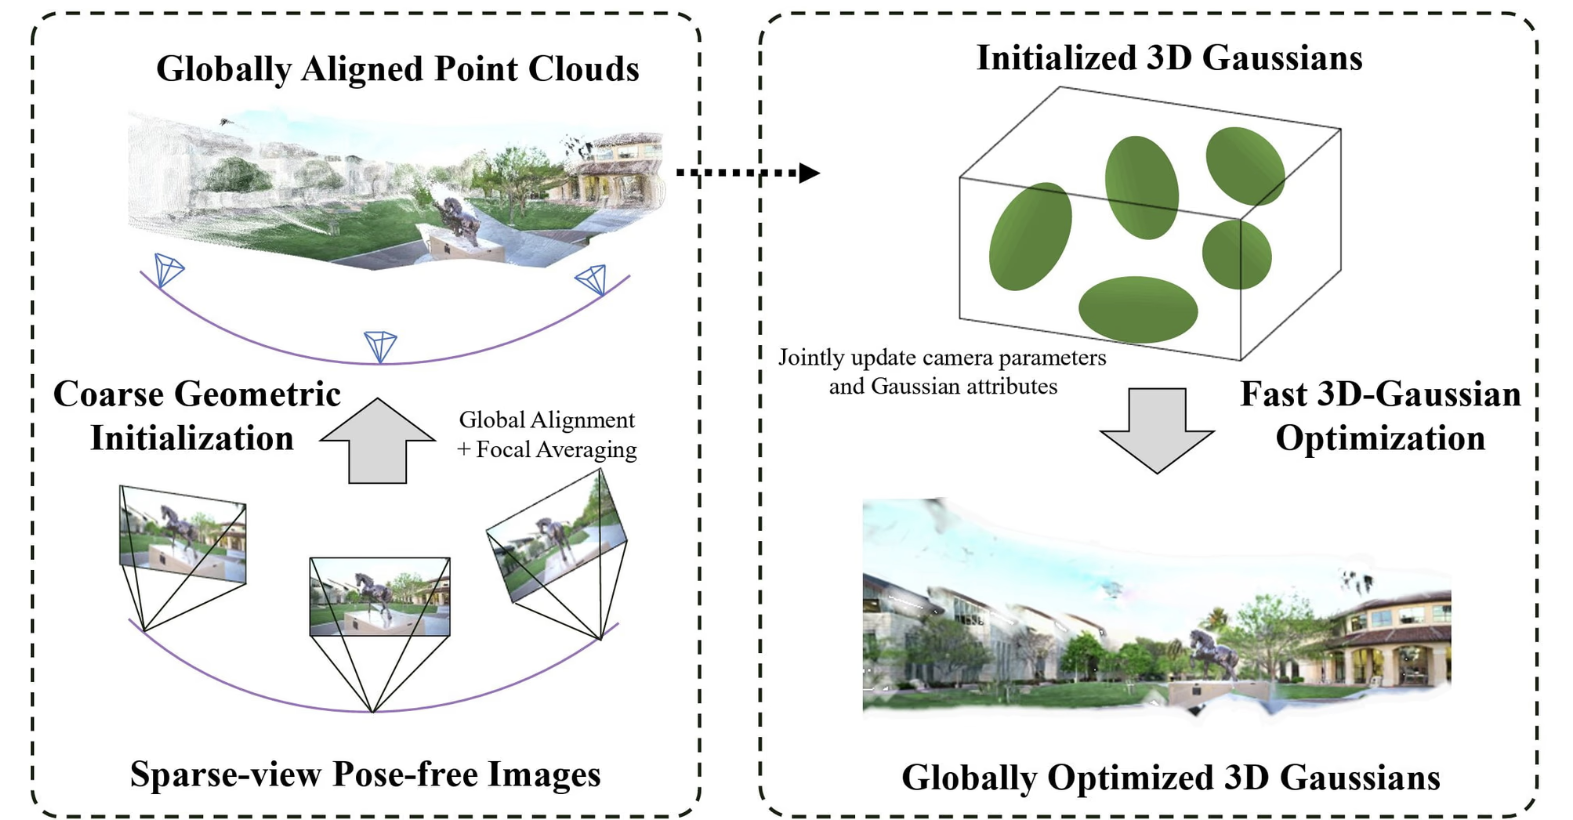
\includegraphics[width=0.8\textwidth]{gaussian_splatting_diagram.png}
      \caption{Gaussian Splatting Visualization: Transforming sparse 3D point clouds into continuous Gaussian distributions.}
      \label{fig:gaussian_splatting}
  \end{figure}

The GSplat framework can be divided into several key components:

\begin{enumerate}
      \item \textbf{GSplat-based Navigation and Mapping:} This involves constructing and refining a representation of the environment using Gaussian splats for real-time navigation. The robot utilizes this representation for pose estimation, path planning, and motion control, allowing it to navigate complex environments safely, this method is much faster than NeRF based representation. As the robot moves through its environment, Gaussian splats are continually refined to ensure accurate mapping and efficient navigation.

      \item \textbf{Image Segmentation and Embeddings:} Beyond navigation, GSplat-based environments enable more advanced perception tasks, such as object detection and semantic understanding. After reconstructing the environment with Gaussian splats, the robot performs image segmentation to identify objects and regions of interest. These segmented regions are converted into high-dimensional image embeddings that capture the essential features of each segment. The image embeddings provide a compact and informative representation of the environment's visual content, facilitating object recognition and other perception tasks.

      \item \textbf{Vector Database Lookup:} The robot stores these image embeddings in a vector database along with their corresponding locations in the point cloud. This database allows for efficient retrieval of similar embeddings, enabling the robot to recognize previously seen objects and environments. By performing vector database lookups during navigation, the robot can recall the semantic information associated with objects and locations, enabling context-aware decision-making.

      \item \textbf{Natural Language Query Processing:} GSplat-based environments also support natural language interactions. The robot can process natural language queries, convert them into embeddings using pre-trained language models, and perform a semantic lookup in the vector database. This allows the robot to answer questions, locate objects, and provide information based on both visual and linguistic inputs. For instance, a query like "Where is the nearest charging station?" will trigger the retrieval of the relevant information from the vector database, enabling the robot to provide accurate responses and assist in complex tasks.

\end{enumerate}

By integrating these components, the GSplat framework combines efficient
real-time navigation with advanced semantic understanding and natural language
processing. This enables robots to perform tasks that go beyond basic
navigation, allowing for meaningful interaction with the environment and
providing valuable contextual information during exploration and task
execution.\cite{KKLD23}

\begin{figure}[h!]
      \centering
      \begin{tikzpicture}[
                  node distance=2.5cm, % Increased node distance
                  every node/.style={font=\small},
                  process/.style={rectangle, draw, minimum width=4cm, minimum height=1cm, rounded corners, align=center},
                  io/.style={trapezium, trapezium left angle=70, trapezium right angle=110, draw, minimum width=4cm, minimum height=1cm, align=center},
                  arrow/.style={thick, ->, >=Stealth}
            ]

            % Nodes
            \node (input) [io] {Sparse Point Cloud};
            \node (reconstruction) [process, below of=input] {GSplat Reconstruction};
            \node (mapping) [process, below of=reconstruction, xshift=-6cm] {GSplat-based\\Mapping}; % Adjusted xshift for more space
            \node (pose) [process, right=0.5cm of reconstruction, below of=reconstruction ] {Pose Estimation}; % Adjusted right shift
            \node (planning) [process, below of=pose] {Path Planning};
            \node (control) [process, below of=planning] {Motion Control};

            % Parallel branch for Image Segmentation, Embeddings, and Vector DB
            \node (segmentation) [process, right=1.5cm of reconstruction] {Image Segmentation}; % Adjusted position
            \node (embedding) [process, below of=segmentation] {Image Embeddings};
            \node (vectorDB) [process, below of=embedding] {Vector Database};

            \node (nlquery) [process, below of=mapping] {Natural Language Query}; % Moved to the bottom left for more space
            \node (nlembedding) [process, below of=nlquery] {Query Embeddings};

            % Arrows
            \draw [arrow] (input) -- (reconstruction);
            \draw [arrow] (reconstruction) -- (pose);
            \draw [arrow] (pose) -- (planning);
            \draw [arrow] (planning) -- (control);
            \draw [arrow] (reconstruction) -- (mapping);

            % Arrows for the parallel branch
            \draw [arrow] (reconstruction) -- (segmentation);
            \draw [arrow] (segmentation) -- (embedding);
            \draw [arrow] (embedding) -- node[anchor=west] {} (vectorDB);

            % Arrows for natural language query
            \draw [arrow] (nlquery) -- (nlembedding);
            \draw [arrow] (nlembedding.south) |- ++(0,-1.5cm) -| node[anchor=west] {Lookup} (vectorDB);

      \end{tikzpicture}
      \caption{GSplat-based Navigation, Mapping, and Semantic Understanding Workflow}
\end{figure}

\section{GSplat-based Navigation and Mapping}

\subsection{GSplat-based Navigation}

\definecolor{codegreen}{rgb}{0,0.6,0}
\definecolor{codegray}{rgb}{0.5,0.5,0.5}
\definecolor{codepurple}{rgb}{0.58,0,0.82}
\definecolor{backcolour}{rgb}{0.95,0.95,0.92}

\lstdefinestyle{mystyle}{
      backgroundcolor=\color{backcolour},
      commentstyle=\color{codegreen},
      keywordstyle=\color{magenta},
      numberstyle=\tiny\color{codegray},
      stringstyle=\color{codepurple},
      basicstyle=\ttfamily\footnotesize,
      breakatwhitespace=false,
      breaklines=true,
      captionpos=b,
      keepspaces=true,
      numbers=left,
      numbersep=5pt,
      showspaces=false,
      showstringspaces=false,
      showtabs=false,
      tabsize=2
}

\lstset{style=mystyle}

\begin{enumerate}
      \item \textbf{GSplat Reconstruction} \\
            Gaussian Splatting initializes the navigation pipeline by transforming a sparse point cloud, obtained via camera calibration or other methods, into 3D Gaussian splats. This reconstruction allows for the environment's geometric representation to be optimized, forming a detailed and efficient basis for real-time navigation tasks. The mathematical representation of a Gaussian splat is given by its mean $\mu \in \mathbb{R}^3$, covariance matrix $\Sigma \in S_{++}$, opacity $\alpha \in [0,1]$, and spherical harmonics coefficients defining view-dependent colors \cite{kerbl20233dgaussiansplattingrealtime}.
            The 3D covariance $\Sigma$ is further decomposed as $\Sigma = R S S^T R^T$, where $R \in SO(3)$ is a rotation matrix and $S$ is a diagonal scaling matrix \cite{chen2024splatnavsaferealtimerobot}.

            To implement the GSplat framework, we utilize a NeRF-based \cite{zhang2024visuallocalization3dmaps} approach provided by
            the `nerfstudio` framework \cite{Tancik_2023}. The following code snippet demonstrates how to
            construct a Gaussian splat model using images from a `data` folder.

            \begin{lstlisting}
      # nerfstudio installation and setup
      pip install nerfstudio
      
      # Prepare your dataset by placing images and camera parameters in the `data` folder
      # The following script initializes the splat model
      
      import nerfstudio as ns
      
      # Path to the dataset
      data_path = "./data"
      
      # Load configuration for the Gaussian Splatting model
      config = ns.configs.get_default_gaussian_splat_config(
            dataset_path=data_path,
            model_name="g_splat_model",
      )
      
      # Instantiate the NeRF Studio pipeline with Gaussian splatting
      pipeline = ns.pipeline.create_pipeline(config)
      
      # Start training the model
      pipeline.train()
      
      # Export the trained splat model for further use in navigation and mapping
      pipeline.save_model("splat_model.pth")
\end{lstlisting}

            This code constructs a Gaussian splatting model from the provided images and
            camera parameters in the `data` folder. The `nerfstudio` framework is leveraged
            to optimize the Gaussian splats for an accurate and efficient environment
            representation. The configuration is automatically managed using the
            \texttt{get\_default\_gaussian\_splat\_config} function, which eliminates the
            need for manual specification of parameters like \texttt{num\_gaussians}.

      \item \textbf{Pose Estimation} \\
            Splat-Loc provides real-time pose estimation by leveraging the point cloud generated from Gaussian splatting. Pose estimation is done using a combination of global initialization and recursive localization based on monocular RGB images. Mathematically, the pose estimation problem can be formulated as a maximum a-posteriori (MAP) optimization problem. Given prior estimates of the robot's pose $\mathbf{x}_{t-1}$ and the measurements $\mathbf{y}_t$, the MAP estimate of the current pose $\mathbf{x}_t$ is computed by minimizing:
            \[
                  \mathbf{x}_t^\star = \arg\min_{\mathbf{x}_t} \left( \| \mathbf{x}_t - f(\mathbf{x}_{t-1}, \mathbf{u}_{t-1}) \|_{Q^{-1}}^2 + \| \mathbf{y}_t - h(\mathbf{x}_t) \|_{R^{-1}}^2 \right)
            \]
            subject to constraints that ensure the pose remains within safe polytope
            corridors defined by the Gaussian splats \cite{bortolon20246dgs6dposeestimation}
            \cite{chen2024splatnavsaferealtimerobot}.

            We are solving the following optimization problem for pose estimation:

            \[
                  x^*_t = \arg \min_{x_t} \left\| x_t - f(x_{t-1}, u_{t-1}) \right\|^2_{Q^{-1}} + \left\| y_t - h(x_t) \right\|^2_{R^{-1}}
            \]

            The Python implementation for this MAP optimization can be written as follows:

            \begin{lstlisting}
import numpy as np
from scipy.optimize import minimize

# Define the state transition function f(x_{t-1}, u_{t-1})
def state_transition(x_prev, u_prev):
    # Example linear transition model
    return np.dot(A, x_prev) + np.dot(B, u_prev)

# Define the measurement function h(x_t)
def measurement_model(x_t):
    # Example measurement model
    return np.dot(C, x_t)

# Define the cost function to minimize
def cost_function(x_t, x_prev, u_prev, y_t, Q_inv, R_inv):
    # State transition error
    state_error = x_t - state_transition(x_prev, u_prev)
    state_cost = np.dot(state_error.T, np.dot(Q_inv, state_error))
    
    # Measurement error
    measurement_error = y_t - measurement_model(x_t)
    measurement_cost = np.dot(measurement_error.T, np.dot(R_inv, measurement_error))
    
    # Total cost
    return state_cost + measurement_cost

# Example matrices (replace with actual values)
A = np.eye(3)  # State transition matrix
B = np.eye(3)  # Control input matrix
C = np.eye(3)  # Measurement matrix
Q_inv = np.eye(3)  # Inverse of process covariance matrix
R_inv = np.eye(3)  # Inverse of measurement covariance matrix

# Previous state, control input, and measurement
x_prev = np.array([1.0, 2.0, 3.0])
u_prev = np.array([0.1, 0.2, 0.3])
y_t = np.array([1.5, 2.5, 3.5])

# Initial guess for the current state
x_t_initial = np.array([1.2, 2.2, 3.2])

# Perform the optimization
result = minimize(cost_function, x_t_initial, args=(x_prev, u_prev, y_t, Q_inv, R_inv))

# Optimal pose estimate
x_t_optimal = result.x
print("Optimal Pose Estimate:", x_t_optimal)
\end{lstlisting}

            This code implements the MAP optimization problem for pose estimation. It uses
            the \texttt{scipy.optimize.minimize} function to find the optimal pose $x_t$ by
            minimizing the cost function, which is a combination of the state transition
            and measurement model errors.

      \item \textbf{Path Planning} \\
            The Splat-Plan module ensures safe navigation through the environment by constructing polytopic safe corridors. These polytopes are created by decomposing the configuration space into occupied and collision-free regions using the intersection of ellipsoidal approximations of the Gaussian splats. The collision-checking algorithm is based on solving generalized eigenvalue problems and can be parallelized for efficiency. Given a set of safe polytopes, the trajectory planning problem is formulated as a quadratic program that minimizes the path length subject to safety constraints:
            \[
                  \min_{\mathbf{c}_i} \sum_{i=0}^{M-1} \|\mathbf{c}_{i+1} - \mathbf{c}_i\|_2^2 \quad \text{subject to } \mathbf{A}\mathbf{c}_i \leq \mathbf{b}
            \]
            where $\mathbf{c}_i$ are the control points of the Bézier curve representing
            the trajectory \cite{chen2024splatnavsaferealtimerobot}.

            The Splat-Plan module ensures safe navigation by constructing polytopic safe
            corridors. These polytopes are created by decomposing the configuration space
            into occupied and collision-free regions using the intersection of ellipsoidal
            approximations of Gaussian splats.

            The trajectory planning problem can be formulated as a quadratic program (QP)
            that minimizes the path length subject to safety constraints:

            \[
                  \min_{\{c_i\}} \sum_{i=0}^{M-1} \left\| c_{i+1} - c_i \right\|^2_2 \quad \text{subject to} \quad A c_i \leq b
            \]

            Here, \( c_i \) are the control points of the Bézier curve representing the
            trajectory. The following Python code implements this optimization problem.

            \begin{lstlisting}
import numpy as np
from scipy.optimize import minimize

# Example quadratic cost function
def trajectory_cost(control_points):
    total_cost = 0
    for i in range(len(control_points) - 1):
        total_cost += np.linalg.norm(control_points[i+1] - control_points[i])**2
    return total_cost

# Example constraint function for the polytope constraints
def polytope_constraints(control_points, A, b):
    constraints = []
    for c_i in control_points:
        constraints.append({'type': 'ineq', 'fun': lambda c_i, A=A, b=b: b - np.dot(A, c_i)})
    return constraints

# Example setup (replace with actual matrices and values)
M = 5  # Number of control points
A = np.array([[1, 0], [0, 1]])  # Example polytope constraint matrix
b = np.array([1, 1])  # Example constraint bounds

# Initial guess for control points (random initialization)
initial_control_points = np.random.rand(M, 2)

# Set up the constraints for all control points
constraints = polytope_constraints(initial_control_points, A, b)

# Perform the optimization (minimizing path length subject to polytope constraints)
result = minimize(trajectory_cost, initial_control_points, constraints=constraints)

# Optimal control points
optimal_control_points = result.x.reshape(M, 2)
print("Optimal Control Points:", optimal_control_points)
\end{lstlisting}

            This code formulates and solves the quadratic program for trajectory planning.
            It minimizes the path length defined by the control points \( c_i \) of a
            Bézier curve, while ensuring that the trajectory remains within the safe
            polytope corridors by enforcing the constraint \( A c_i \leq b \).

      \item \textbf{Motion Control} \\
            The planned trajectory is executed through motion control algorithms that ensure smooth and precise movement of the robot. \cite{DURAKLI2022101540} The trajectory is generated using Bézier curves within the safe polytopes, which guarantees safety and efficiency. The motion control system is integrated with the Gaussian splatting environment, allowing for dynamic adjustments in real-time navigation.

\end{enumerate}

\subsection{GSplat-based Mapping}
\begin{enumerate}
      \item \textbf{GSplat Reconstruction} \\
            For mapping, Gaussian Splatting is used to optimize the representation of 3D Gaussians, which enables efficient storage and real-time updates to the map. The anisotropic covariance matrices are adjusted to balance between map detail and computational efficiency \cite{kerbl20233dgaussiansplattingrealtime}.

      \item \textbf{Exploration and Mapping} \\
            Robots using Gaussian Splatting can perform continuous exploration and mapping, adjusting their internal representation of the environment as they move. The exploration is driven by the robot's need to maintain an updated understanding of the surroundings, avoiding obstacles while generating a detailed map.

      \item \textbf{Map Refinement} \\
            Gaussian splats are refined by adjusting their anisotropic covariances as the robot gathers more data from the environment. This allows for the continuous refinement of the environment representation, ensuring that the robot's map remains accurate and precise over time \cite{kerbl20233dgaussiansplattingrealtime}.

\end{enumerate}

\section{Semantic Understanding and Knowledge Retrieval in GSplat Environments}

The continuous environment representation created by Gaussian splatting is
leveraged for more advanced tasks, including semantic understanding,
image-based query processing, and natural language queries. These processes
enable robots to interact more meaningfully with their surroundings by
providing both perceptual and cognitive capabilities.\cite{che2024enhancingmultimodalunderstandingclipbased}

\subsection{Image Segmentation and Embeddings}

After the environment has been reconstructed using Gaussian splatting, the
robot performs image segmentation to identify objects and regions of interest
within its field of view. Image segmentation divides the visual input into
segments corresponding to distinct objects or surfaces, helping the robot to
parse the environment into meaningful components. \cite{ravi2024sam}

Once the image segmentation process is complete, the segmented regions are
passed through a neural network to generate high-dimensional image embeddings.
These embeddings represent the visual content in a compact form, capturing the
essential features of each segment. The embeddings are crucial for both object
recognition and later retrieval tasks. \cite{che2024enhancingmultimodalunderstandingclipbased}

\begin{figure}[h]
      \centering
      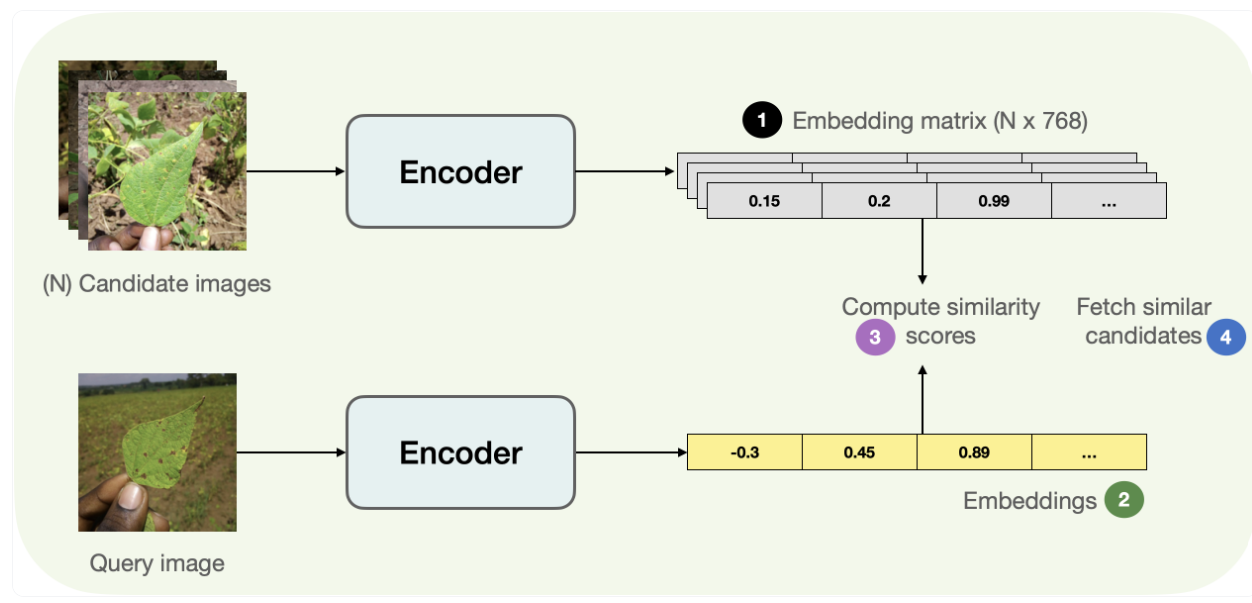
\includegraphics[width=\textwidth]{embeddings.png} % Adjust the width as necessary
      \caption{Image Embeddings for Semantic Understanding} % Caption for the image
      \label{fig:embeddings} % Label for referencing the image
\end{figure}

\subsection*{1. Convert Image to Embeddings}

We use the CLIP model from the `transformers` library to convert images into
embeddings.

\begin{lstlisting}
from transformers import CLIPProcessor, CLIPModel
from PIL import Image
import torch

# Load a pre-trained CLIP model and processor
model = CLIPModel.from_pretrained("openai/clip-vit-base-patch32")
processor = CLIPProcessor.from_pretrained("openai/clip-vit-base-patch32")

# Function to convert an image to embeddings
def image_to_embeddings(image_path):
    image = Image.open(image_path)
    inputs = processor(images=image, return_tensors="pt")
    with torch.no_grad():
        embeddings = model.get_image_features(**inputs)
    return embeddings.squeeze().numpy()

# Example usage
image_path = "example_image.jpg"
image_embeddings = image_to_embeddings(image_path)
print("Image Embeddings:", image_embeddings)
\end{lstlisting}

\subsection*{2. Store Embeddings in ChromaDB}

After converting the image to embeddings, we store the embeddings in ChromaDB which uses FAISS  to lookup similar embeddings efficiently. \cite{douze2024faisslibrary},
a vector database for efficient storage and retrieval of embeddings.

\begin{lstlisting}
import chromadb
from chromadb.utils import embedding_store

# Initialize ChromaDB client
client = chromadb.Client()

# Create a collection to store embeddings
collection = client.create_collection("multimodal_embeddings")

# Function to store embeddings in ChromaDB
def store_embeddings(id, embeddings, metadata=None):
    collection.add(id=id, embedding=embeddings.tolist(), metadata=metadata)

# Store the image embeddings with an identifier
store_embeddings(id="image_1", embeddings=image_embeddings, metadata={"type": "image"})
\end{lstlisting}

\subsection*{3. Convert Text Query to Embeddings}

We convert a text query into embeddings using the same CLIP model, allowing for
multimodal comparisons. \cite{che2024enhancingmultimodalunderstandingclipbased}

\begin{lstlisting}
# Function to convert text query to embeddings
def text_to_embeddings(text_query):
    inputs = processor(text=text_query, return_tensors="pt")
    with torch.no_grad():
        embeddings = model.get_text_features(**inputs)
    return embeddings.squeeze().numpy()

# Example usage
text_query = "A cat sitting on a chair"
text_embeddings = text_to_embeddings(text_query)
print("Text Query Embeddings:", text_embeddings)
\end{lstlisting}

\subsection{Vector Database Lookup}

The image embeddings generated from the segmented regions are stored in a
vector database along with their associated locations in the point cloud. The
vector database enables fast and efficient retrieval of similar embeddings,
facilitating object recognition, tracking, and semantic labeling.

During navigation, if the robot encounters a previously observed region or
object, it can perform a vector database lookup by comparing the current image
embeddings with the stored embeddings. This comparison allows the robot to
recognize familiar objects and recall their previously associated semantic
labels, enabling context-aware decision-making and interaction with the
environment.\cite{douze2024faisslibrary}

\begin{lstlisting}
      # Function to lookup similar embeddings in ChromaDB
      def query_similar_embeddings(embeddings, top_k=5):
          results = collection.query(embedding=embeddings.tolist(), n_results=top_k)
          return results
      
      # Query similar embeddings using the text query embeddings
      similar_embeddings = query_similar_embeddings(text_embeddings)
      print("Similar Embeddings:", similar_embeddings)
      \end{lstlisting}

\subsection{Natural Language Query Processing}

In addition to image-based processing, the robot is capable of understanding
and processing natural language queries. The process begins with the robot
receiving a natural language query, such as "Where is the nearest charging
station?" or "Identify the red object in the room."

The query is first converted into a high-dimensional embedding using a
pre-trained language model. This embedding captures the meaning of the query
and is used to perform a semantic lookup in the vector database. The robot
compares the query embedding with the stored image embeddings and retrieves the
relevant objects or locations that match the query.

For example, if the query is about finding a specific object, the robot will
locate the corresponding image embeddings in the vector database and return the
object's location in the point cloud. This allows the robot to answer questions
about its environment and provide meaningful responses based on its prior
knowledge and observations. \cite{che2024enhancingmultimodalunderstandingclipbased}

\subsection{Integration with Navigation and Mapping}

The semantic understanding and query processing capabilities are integrated
with the GSplat-based navigation and mapping pipeline. As the robot explores
its environment, it continuously updates its internal representation with new
Gaussian splats, image embeddings, and semantic labels. This enables the robot
to build a rich and detailed map of the environment that can be queried both
visually and linguistically.

Furthermore, the vector database provides a way to efficiently store and
retrieve this information, allowing the robot to recognize objects and
locations that it has previously encountered. This integration ensures that the
robot can perform advanced navigation tasks while maintaining an updated
understanding of its surroundings.

By combining Gaussian splatting with image segmentation, embeddings, and
natural language processing, the robot can achieve a high level of semantic
understanding, enabling it to interact with complex environments in a
meaningful and intelligent way.

